\chapter{Restauração de Imagens Usando Super-resolução}
\label{chap:superRes}
\section{Introdução}
Entende-se por Super-resolução o processo de obtenção de uma ou mais imagens de alta resolução a partir de uma ou mais imagens de baixa resolução.
Técnicas de super-resolução são pesquisadas desde os anos 1970 e têm despertado um grande interesse de estudo nas últimas décadas.
As aplicações de técnicas de SR são diversas e incluem aprimoramentos de imagens médicas, de imagens de rosto, de texto e impressões digitais \cite{nasrollahi2014super}.

Vale esclarecer que, neste trabalho, sempre que a palavra \textit{resolução} é usada,
ela se refere à resolução espacial de uma imagem, a qual mede a densidade de pontos por
unidade de área em uma imagem \cite{zibetti2007super}.

Este capítulo fará uma breve síntese do histórico das técnicas de super-resolução e seus
principais exemplares.
A Seção \ref{sec:obsmodel} descreve o modelo de observação usado pelos principais
trabalhos no tema. A Seção \ref{sec:srmetodos} cita e descreve resumidamente as
principais técnicas e grupos de métodos de restauração de imagens via super-resolução. 

\section{\label{sec:obsmodel}Modelo de Observação}


Definir um modelo de observação que relacione a imagem de alta resolução às imagens
de baixa resolução observadas é fundamental para o desenvolvimento de qualquer técnica
de super-resolução. Um modelo de observação permite parametrizar e quantificar as
transformações às quais a imagem é submetida durante o processo de aquisição e é
através dele que os principais métodos de super-resolução inferem as características
da imagem de alta resolução.

O modelo de observação deste trabalho simula cinco tipos de alteração aplicadas por
sistemas de aquisição de imagens, a saber: rotação, deslocamento, espalhamento de
ponto, subamostragem e ruído.
Este modelo de observação é descrito tanto no artigo de Tipping
\cite{tipping2003bayesian} quanto em outros trabalhos relacionados
\cite{pickup2007bayesian, Capel01a}.

As alterações de deslocamento linear e rotação tentam simular um possível movimento
aleatório da câmera em relação ao objeto ou vice-versa.
A transformação de espalhamento de ponto simula um efeito de desfoque causado por um
desajuste na definição de foco da câmera.
A subamostragem representa a perda de resolução espacial aplicada à imagem captada
por um sensor CMOS ou CCD de densidade menor do que a necessária para registrar os dados da imagem sem que ocorra \emph{aliasing}.
A Figura \ref{fig:image_transformations} ilustra o efeito destas cinco transformações em uma imagem.

\begin{figure}[h]
	\centering
	\caption{\label{fig:image_transformations}Ilustração demonstrado as transformações sofrida por uma imagem durante o processo de aquisição.}
	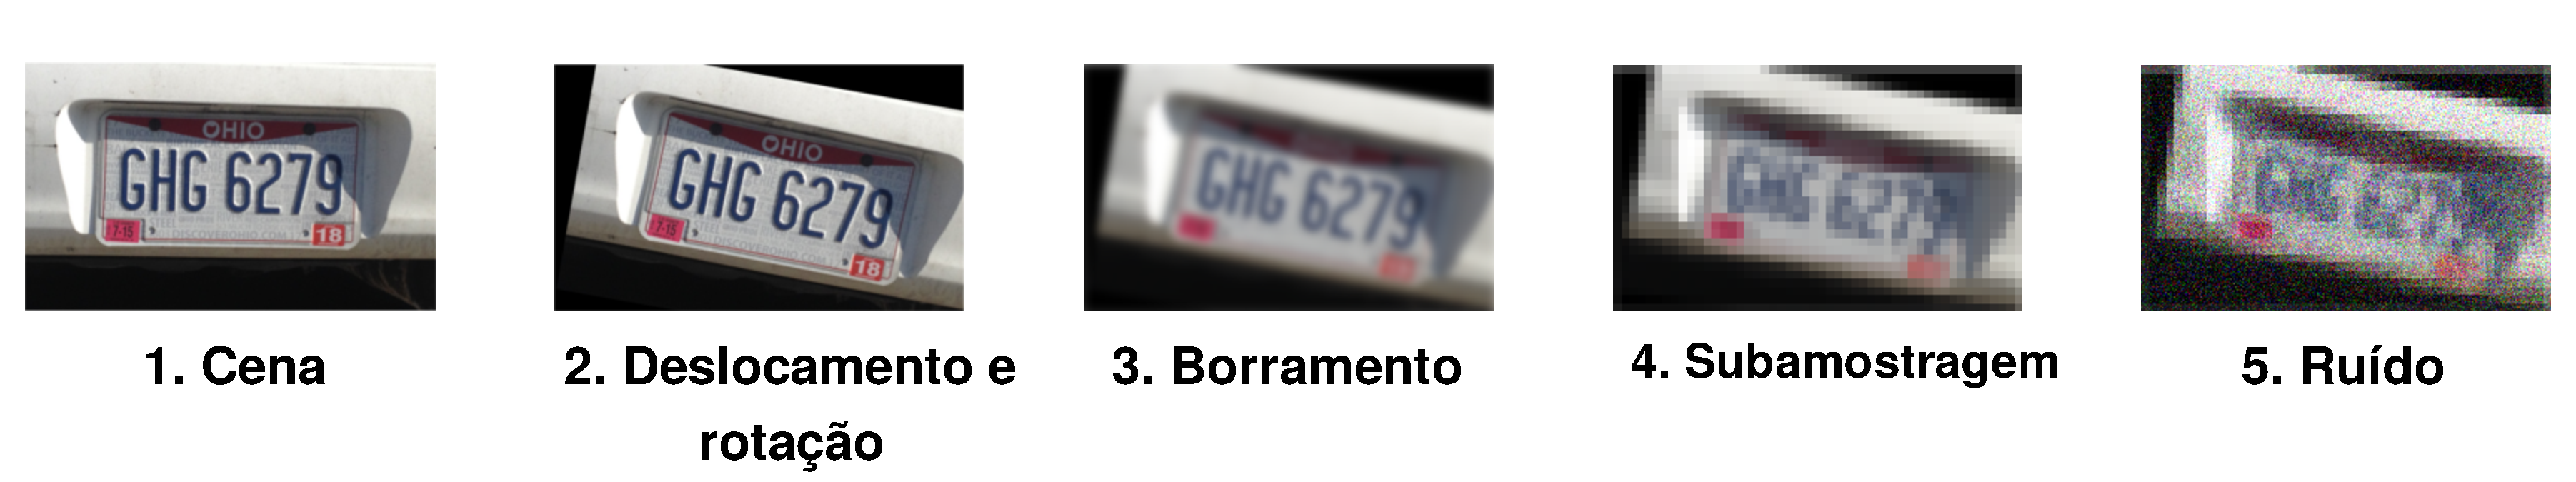
\includegraphics[width=0.95\textwidth]{./figures/image_transformations.pdf}
	\legend{Fonte: O autor.}
\end{figure}

Pela conveniência do modelo de observação, a imagem de alta resolução de dimensões $m \times n$ é representada por um vetor coluna $\mathbf{x} = [x_1, x_2, ... , x_{N-1}, x_N]^T$ onde $N ={} m \times n$. Ou seja, os valores dos pixels da imagem são rearranjados em um vetor de comprimento $N$.

Sabendo disso, a relação entre uma imagem de alta resolução $\mathbf{x}$ e uma imagem degradada $\mathbf{y}^{(k)}$ é resumida em (\ref{eq:degradation}). Onde $k = 1,2,...,K$; sendo $K$ o número total de quadros obtidos a partir da cena de alta resolução $\mathbf{x}$.

\begin{equation}
	\label{eq:degradation}
	\mathbf{y}^{(k)} = \mathbf{W}^{(k)}\mathbf{x} + \mathbf{n}^{(k)}
\end{equation}

O ruído, representado por $\mathbf{n}$ é um vetor de variáveis aleatórias Gaussianas independentes de média zero e variância $1/\beta$.

A matriz de sistema $\mathbf{W}$ aplica as transformações de rotação, deslocamento, subamostragem e espalhamento de ponto ao ser multiplicada pela imagem de alta resolução $\mathbf{x}$.
Pelas propriedades da multiplicação de matrizes, é natural que as dimensões da matriz de sistema sejam $M \times N$; onde $M$ é o número de pixels da imagem resultante.
Também se espera que $N \gg M$.

A matriz $\mathbf{W}$ depende de três parâmetros de transformação: a largura da função de espalhamento de ponto $\gamma$, um ângulo de rotação $\theta$ e um vetor de deslocamento linear $\mathbf{s}$.
Os elementos da matriz são dados por (\ref{eq:wmatrix}) com a função de espalhamento de ponto descrita em (\ref{eq:psf}) enquanto os parágrafos seguintes demonstram como as demais transformações são incorporadas à matriz de sistema.

\begin{gather}
	\label{eq:wmatrix}
	W^{(k)}_{ji} = \widetilde{W}^{(k)}_{ji} / \sum_{i'} \widetilde{W}^{(k)}_{ji} \\
	\label{eq:psf}
	\widetilde{W}^{(k)}_{ji} = \exp \left\{- \frac{\|\mathbf{v}_i - \mathbf{u}^{(k)}_j\|^2}{\gamma^2} \right\}
\end{gather}

Os vetores $\mathbf{u}^{(k)}_j$ representam o centro da função de espalhamento de ponto e é descrito em (\ref{eq:psfcenter}).
Caso não houvesse espalhamento de ponto, as coordenadas $\{\mathbf{u}_1, \mathbf{u}_2,\mathbf{u}_3,..., \mathbf{u}_M\}$ seriam os pontos de amostragem da imagem de baixa resolução na imagem de alta resolução.
A Figura \ref{fig:transformations} mostra como se dá o processo de subamostragem e outras transformações bidimensionais.

\begin{equation}
	\label{eq:psfcenter}
	\mathbf{u}^{(k)}_j = \mathbf{R}^{(k)}(\mathbf{v}_j-\mathbf{\overline{v}})+\mathbf{\overline{v}}+\mathbf{s}_k
\end{equation}

\begin{equation}
	\mathbf{R}^{(k)} = 
	\begin{pmatrix}
		\cos \theta_k & \sin \theta_k \\
		- \sin \theta_k & \cos \theta_k
	\end{pmatrix}
\end{equation}

\begin{figure}[h]
	\centering
	\caption{\label{fig:transformations}Visualização das transformações de subamostragem, deslocamento linear e rotação.}
	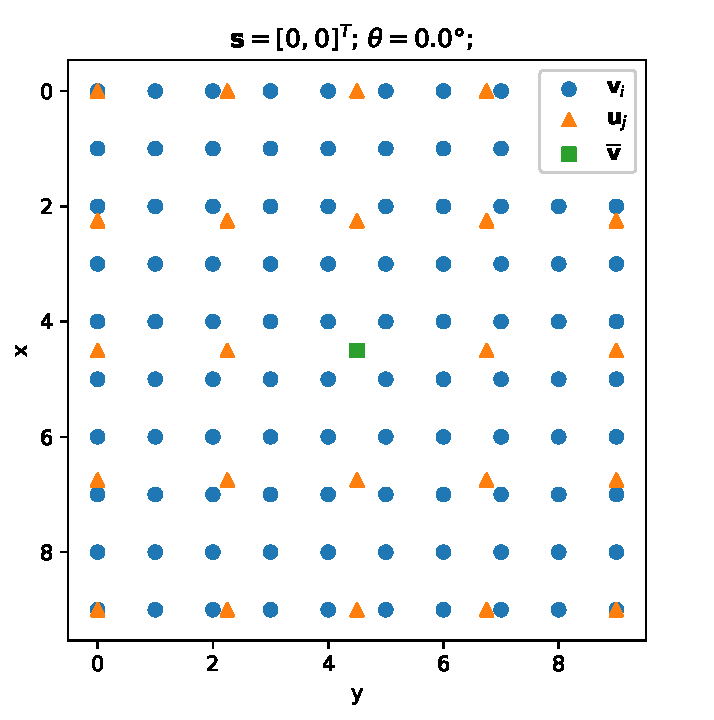
\includegraphics[width=0.3\textwidth]{./figures/transform1.pdf}
	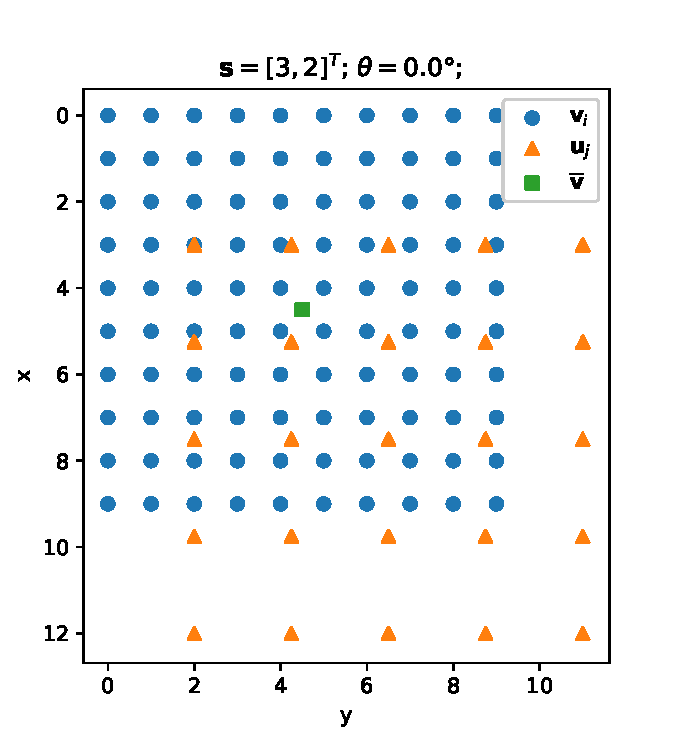
\includegraphics[width=0.3\textwidth]{./figures/transform2.pdf}
	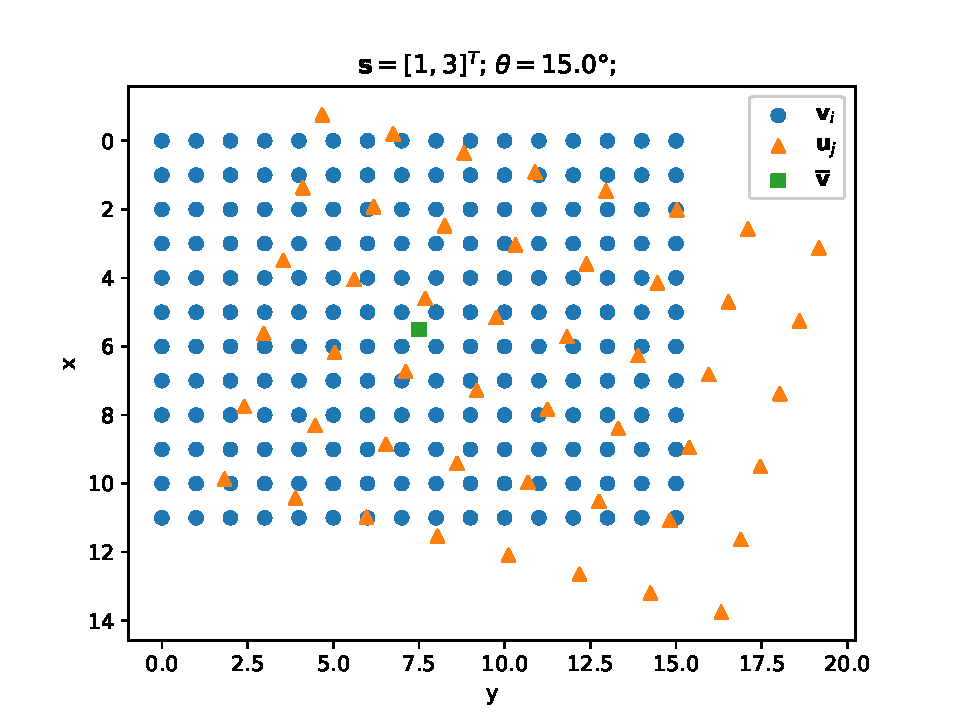
\includegraphics[width=0.3\textwidth]{./figures/transform3.pdf}
	\legend{Fonte: O autor.}
\end{figure}

\begin{figure}[H]
	\centering
	\caption{\label{fig:psfplot}Exemplo de gráfico de uma função de espalhamento de ponto com $\gamma = 2$ centrada em $[0,0]$.}
	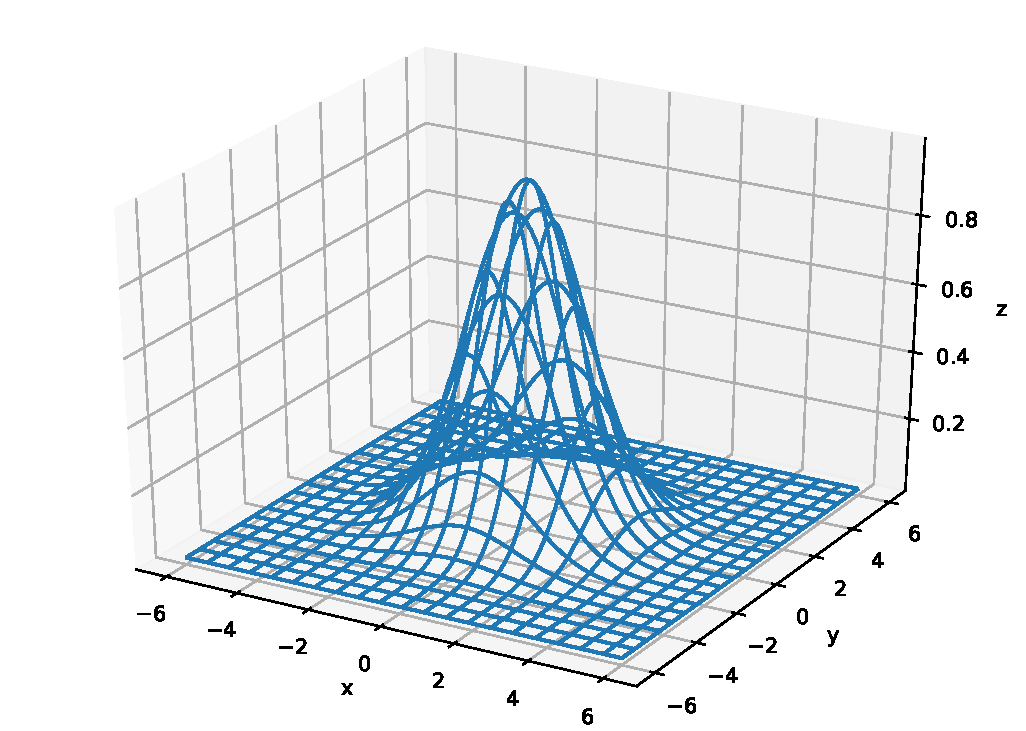
\includegraphics[width = 0.5\textwidth]{./figures/psf1.pdf}
	\legend{Fonte: O autor.}
\end{figure}

A transformação de espalhamento de ponto ou borramento consiste em realizar uma convolução da imagem com uma função gaussiana bidimensional como a mostrada na Figura \ref{fig:psfplot}.
Visualmente, o efeito dessa convolução é equivalente ao de um desfoque de lente, como demonstrado na Figura \ref{fig:psfexample}

\begin{figure}[H]
	\centering
	\caption{\label{fig:psfexample}Exemplo de convolução de uma imagem com uma função de espalhamento de ponto.
	Neste caso, a imagem da direita é resultado da convolução da imagem da esquerda com uma função de espalhamento de ponto gaussiana com $\gamma = 10$.}
	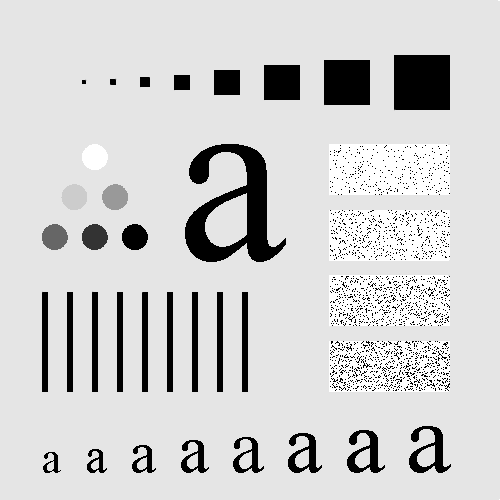
\includegraphics[width = 0.25\textwidth]{./figures/psfexample0.png}
	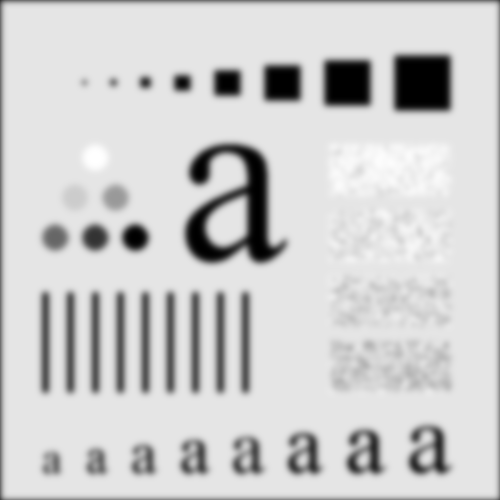
\includegraphics[width = 0.25\textwidth]{./figures/psfexample1.png}
	\legend{Fonte: O autor.}
\end{figure}

